\subsection{Throughput percibido en funcion del tamaño de archivo}

En esta sección vamos a analizar la velocidad de tranmisión de diversos archivos a través de una red local utilizando el protocolo PTC. Para ello montamos un server en determinada máquina, llamémosla A y, un cliente, B, en otra máquina de la misma red. Antes de poder comenzar el envío de datos es necesario que tanto A como B establezcan una conexión entre si. Esto se realiza a través de un algoritmo $three-way \ handshake$ implementando en PTC. Una vez establecida la conexión, B envía varios archivos de distintos tamaños y, por cada archivo, calcula el tiempo insumido en realizar dicha acción para luego calcular el $throughput$. En definitiva, lo que hacemos es setear un timer que arranca cuando se comienza a enviar un archivo desde B y se detiene cuando A le informa que llegó satisfactoriamente. Luego, dividimos el tamaño del archivo enviado (en Bytes) por el tiempo insumido (s) y lo multiplicamos por 1024 para obtener la velocidad en Kb/s.

Analizaremos el $throughput$ percibido en función del tamaño de los archivos enviados testeándolo en diversos entornos. Tomaremos tres tipos de entorno posibles:
\begin{itemize}
	\item[1] Entorno sin delay agregado en los ACK's y con probabilidad 0 de que se pierdan paquetes.
	\item[2] Entorno con delay agregado que se va modificando dinámicamente entre 20ms y 80ms con probabilidad 0 de pérdida de paquetes.
	\item[3] Entorno con delay agregado que se va modificando dinámicamente entre 20ms y 80ms con probabilidad 0.05 de pérdida de paquetes.
\end{itemize}

A continuación, los resultados:

\begin{figure}[H]
	\begin{center}
		  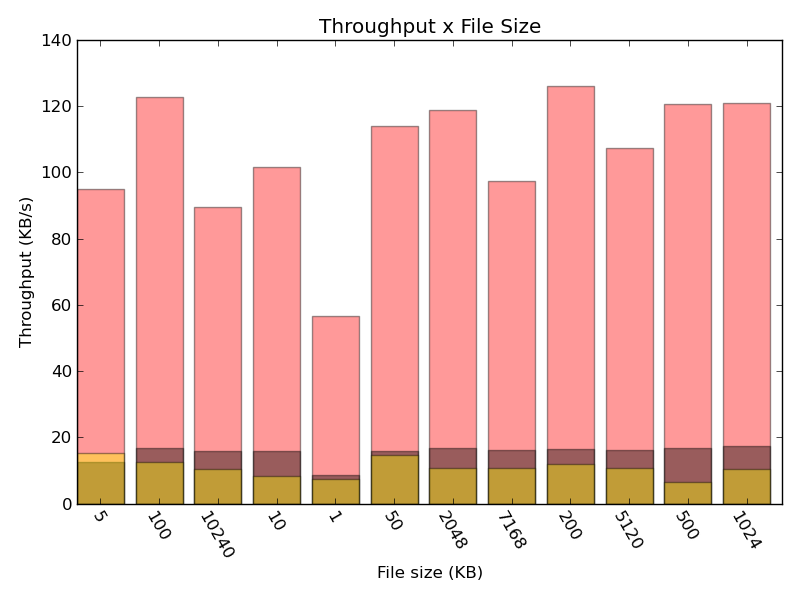
\includegraphics[scale=0.5]{../graficos/test1_1.png}
		  \caption{$Throughput$ en cada entorno en función del tamaño del archivo}
		  \label{fig:contra1}
	\end{center}
\end{figure}

Viendo los resultados obtenidos concluimos en que mientras más 'real' es el entorno peor es el $throughput$ percibido y esto es algo que intuitivamente se esperaba. Si transferimos archivos en un entorno sin delay cuya pérdida de paquetes tiene probabilidad 0 es esperable que tenga una velocidad mucho mayor que en una donde si hay delay y pérdida de paquetes. Esto se ve claramente entre el entorno 1 y 2 y el entorno 1 y 3. La diferencia no es tan grande entre los entornos 2 y 3, en donde la única diferencia es la probabilidad de pérdida de paquetes.

Otro punto a analizar es el $throughput$ en función del tamaño del archivo para cada entorno. Si bien hay diferencia en la velocidad de transmisión para cada archivo esta se mantiene bastante parecida entre todos ellos. El único $throughput$ que difiere bastante es el del archivo de 1KB. Sin embargo debemos tener en cuenta de que se trata de un archivo muy pequeño y cuyo tamaño es igual al del Receive Buffer Size. Por este motivo no debemos darle tanta importancia a ese valor.

\subsection{Transferencia de 100 archivos de 1KB vs 1 archivo de 100KB}

Nos pareció interesante comparar el $throughput$ para 100 archivos de 1KB con el de 1 archivo de 100KB. Los resultados fueron 0.29Kb/s en el caso de los 100 archivos de 1kb y 10,86Kb/s para el archivo de 100KB. Cabe aclarar que el experimento se desarrollo en el entorno 3.

Es razonable haber obtenido una diferencia tan grande entre ambas transferencias ya que para enviar 100 archivos de 1KB el cliente debe interactuar con el server cada vez que desea enviar un nuevo archivo y especificarle el tamaño del mismo con el mini protocolo que implementamos. Esto no sucede en el otro caso ya que solo le especifica al server una vez de que tamaño va a ser el archivo a enviar.
